\newcommand{plcchart}{Logic Control Charts}
%Introduction to state charts
\section{Overview of State Charts} \label{sec:overviewstatechart}

Our proposed visual programming language involves using directed state charts with guarded edges. Our languages differs in a few concepts from the usual state charts syntax in order to support features of the hardware. To better understand these differences we will first introduce all the syntax and semantics of a standard UML based state chart.

A State Chart\cite{StateChartVis} is generally defined as a diagram describing the behaviour of a discrete system. Such systems are usually finite state machines. 

%http://en.wikipedia.org/wiki/State_diagram (find different source Taylor atomata paper
Mathematically a state chart can be defined as $M = \lbrace Q, \Sigma, Z, \delta, q_0, F \rbrace$

\begin{definition}
State Charts

\begin{itemize}
	\item \textbf{Q:} Set of states.
	\item \textbf{$\Sigma$:} Set of input symbols or actions, these are used when checking guard conditions.
	\item \textbf{G:} Set of guard conditions $R \times \sigma \rightarrow Boolean$.
	\item \textbf{Z:} Set of output symbols generated by the system.
	\item \textbf{$\delta$:} Set of state transitions with the mapping $\omega: \Sigma \times Q \times G \rightarrow Q$. These are drawn as arrows and are immediately taken if their guard conditions are true.
	\item \textbf{$q_0$:} $q_0 \in Q$ Starting state, can be defined as an initial state with no incoming transitions.
%% Accepting states removed as they are not required for standard states.
%%	\item \textbf{F:} Accepting states for the system, can also sometimes represent the final state. Drawn as a double outline to the state symbol.
\end{itemize}
\end{definition}

A state can be thought of as a set of operating conditions that for example in figure \ref{fig:state_blink_light}
one such state the light is on.

\begin{figure}[htp]
    \centering
    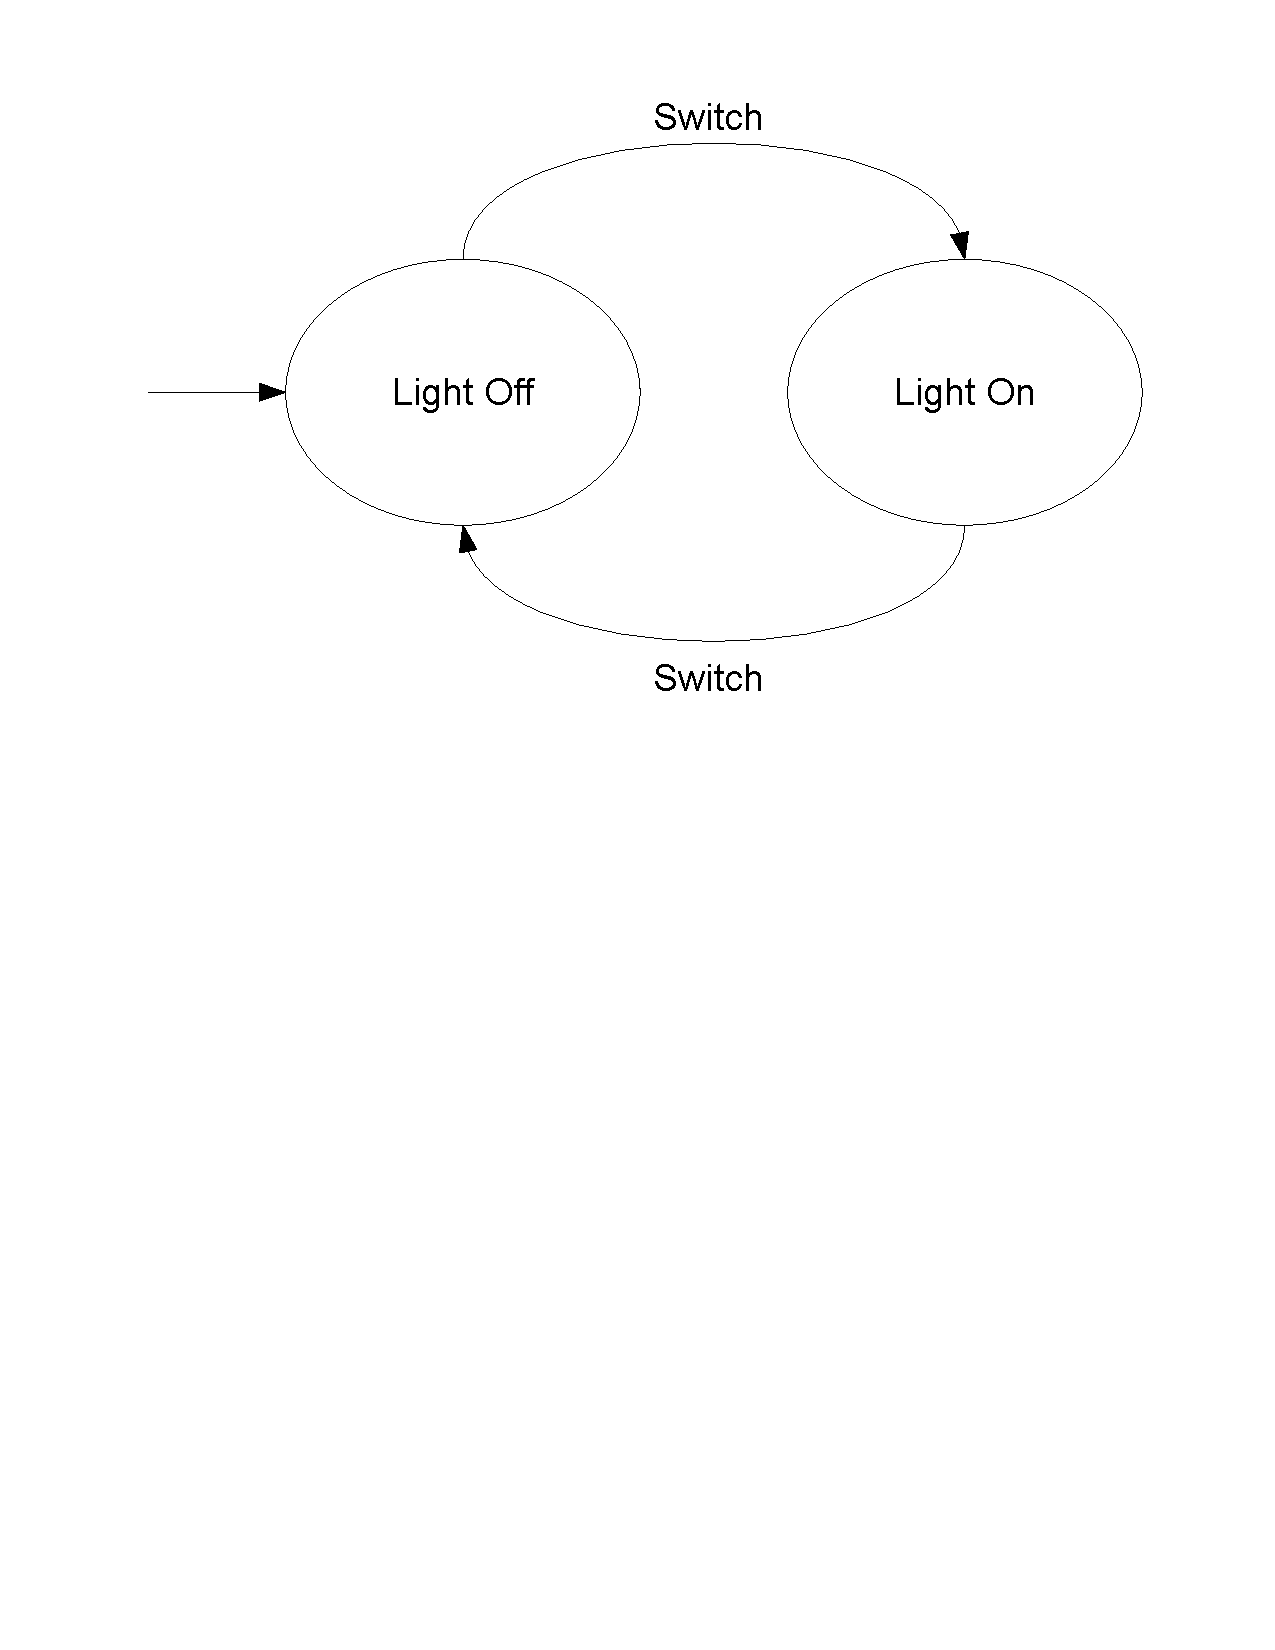
\includegraphics[trim= 10mm 150mm 10mm 10mm, clip, width=\imgmedium]{./images/state_blink_light.pdf}
    \caption{Simple Toggle Light}
    \label{fig:state_blink_light}
\end{figure}

We observe that transitions must always be connected on the tail end and the tip to a state. In addition if a transition can be taken it must be taken immediately. Transitions may also have a guard condition associated with them. If a guard condition does not exist then it is assumed the transition can always be taken. In addition to a guard condition each transition may have an output associated with them. Moore style state machines do not contain outputs on transition edges, Mealy machines do contain an extra output per transition (see: figure \ref{fig:state_moore_mealy}). The output edge on a Mealy machine are denoted by a "/" symbol. Although figure \ref{fig:state_moore_mealy} contains outputs for all edges, we can define ourselves a null output or a no change output in order to simulate an edge having no output as well. For purposes of \plcchart language we do not require the power of a Mealy machine and thus we chose to stay with a simpler Moore machine. More details of this decision can be found in the language section \ref{sec:lang:statesemantics} State Chart Semantics.

%diagram for Moore + Mealy state machines
\begin{figure}[htp]
    \centering
    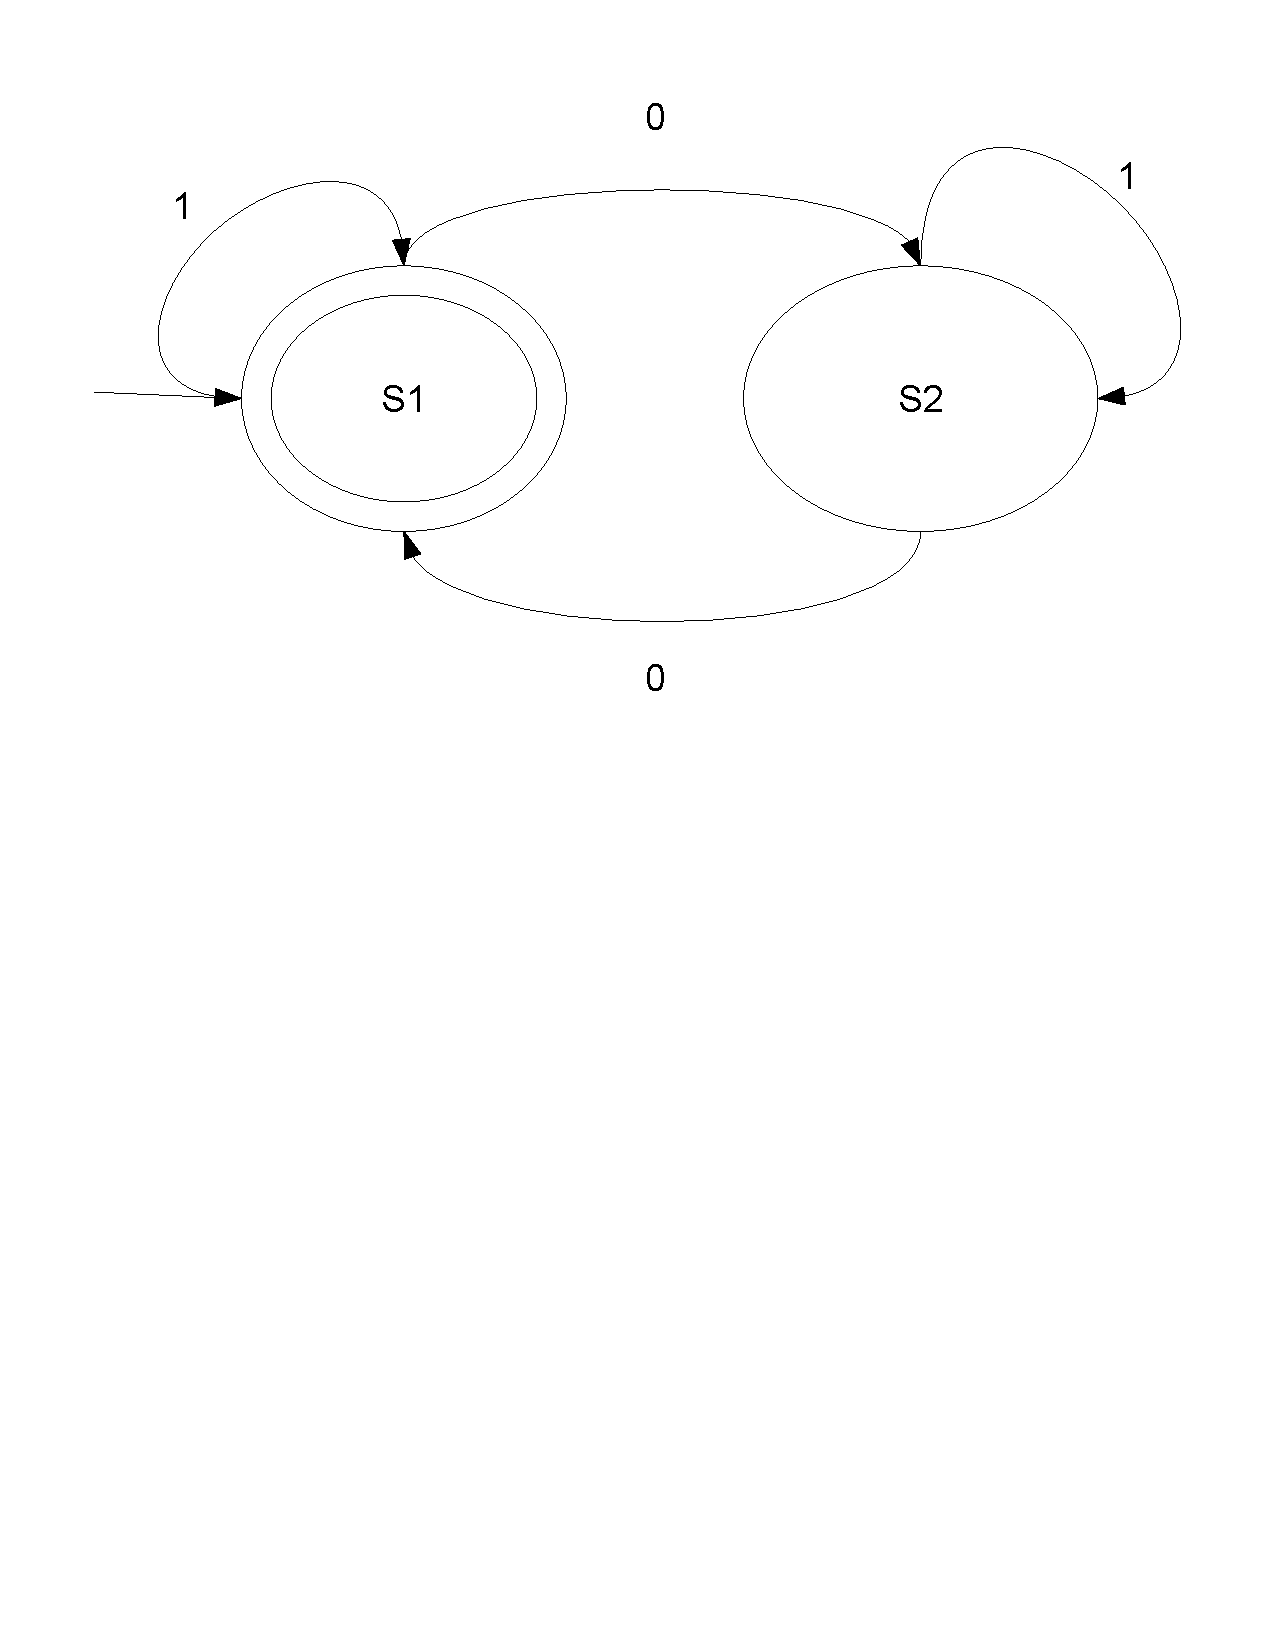
\includegraphics[trim= 15mm 150mm 15mm 10mm, clip, width=200pt]{./images/state_moore.pdf} 
    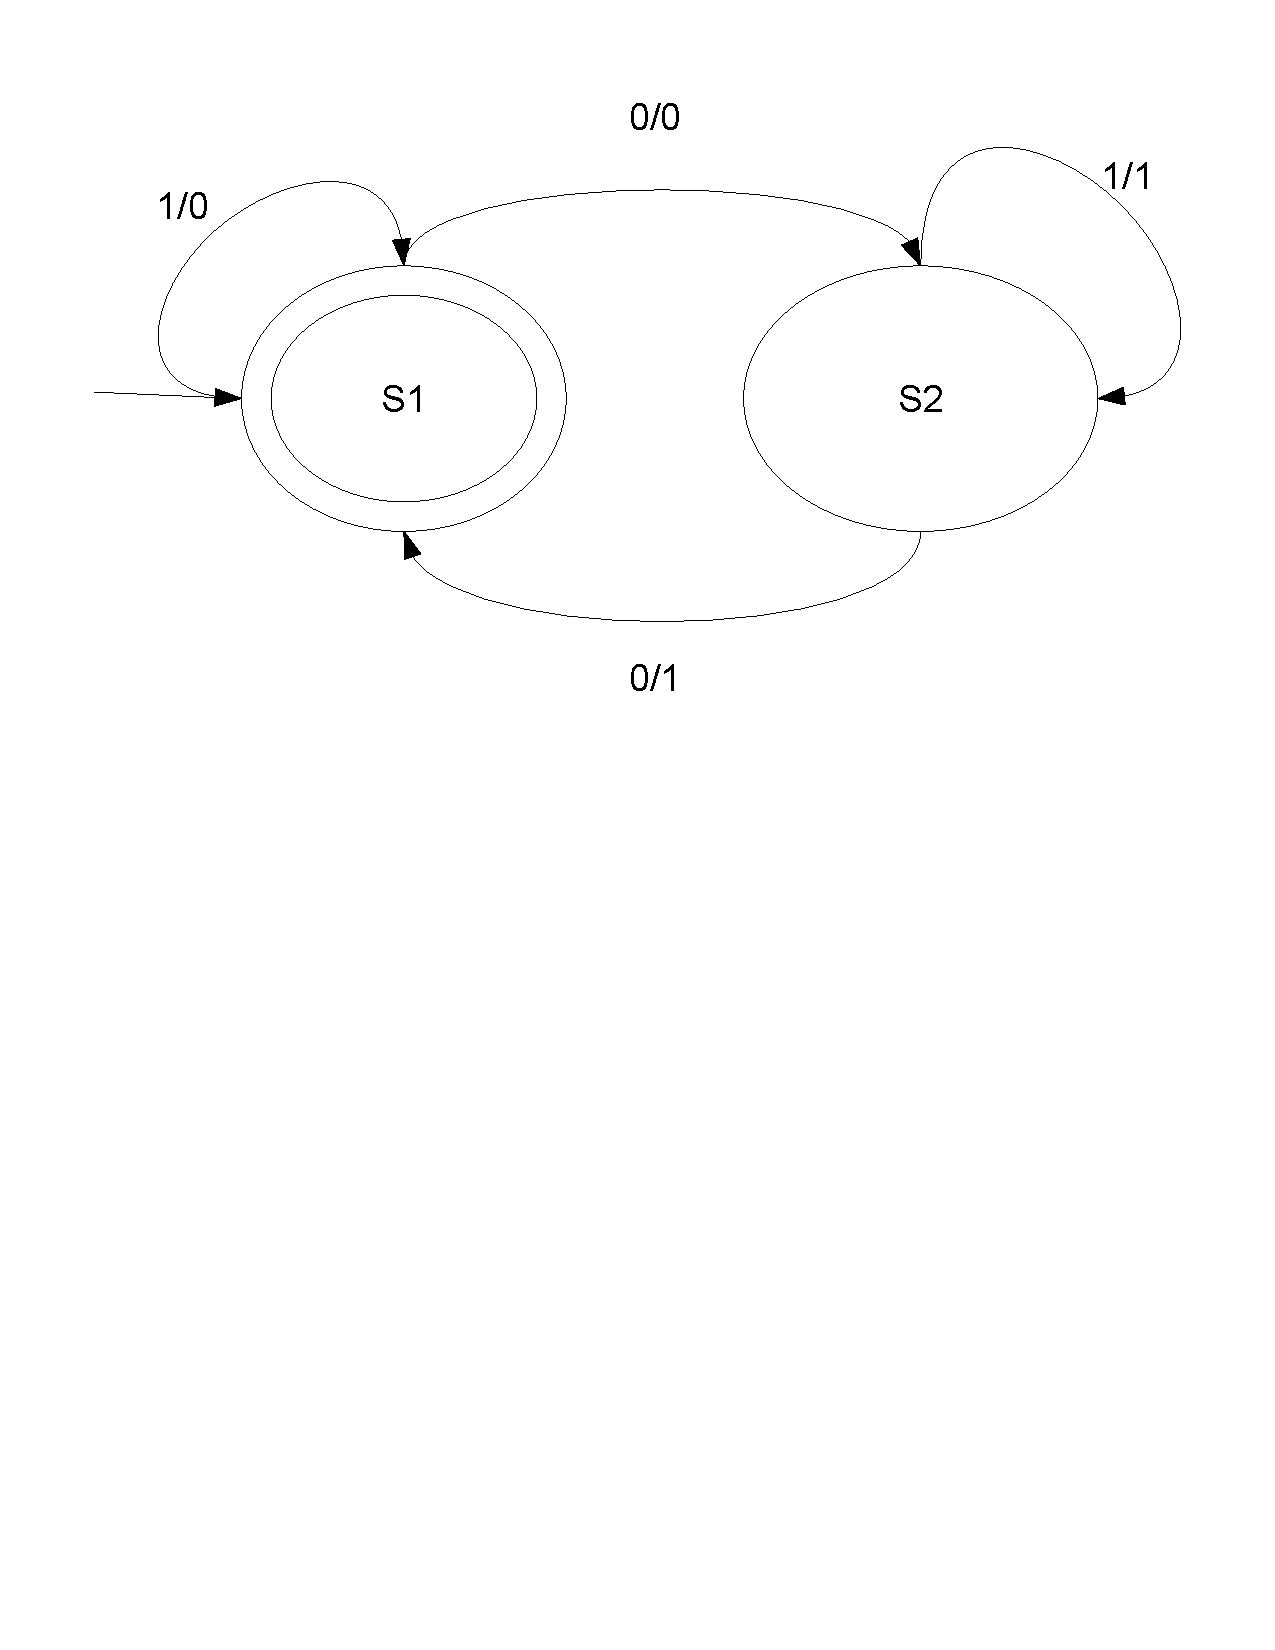
\includegraphics[trim= 15mm 150mm 15mm 10mm, clip, width=200pt]{./images/state_mealy.pdf}    
    \caption{Moore and Mealy State Machines}
    \label{fig:state_moore_mealy}
\end{figure}

There are several ways a starting state can be defined as seen in figure \ref{fig:state_moore_mealy}.
One such way is to draw a edge that has no state connected to its tail, this generally looks like an edge out of nowhere. In our system we choose to use the UML symbol where the start state edge has a solid dot connected to the tail as shown in figure \ref{fig:state_uml_light}.

%diagram for UML state machines
\begin{figure}[htp]
    \centering
    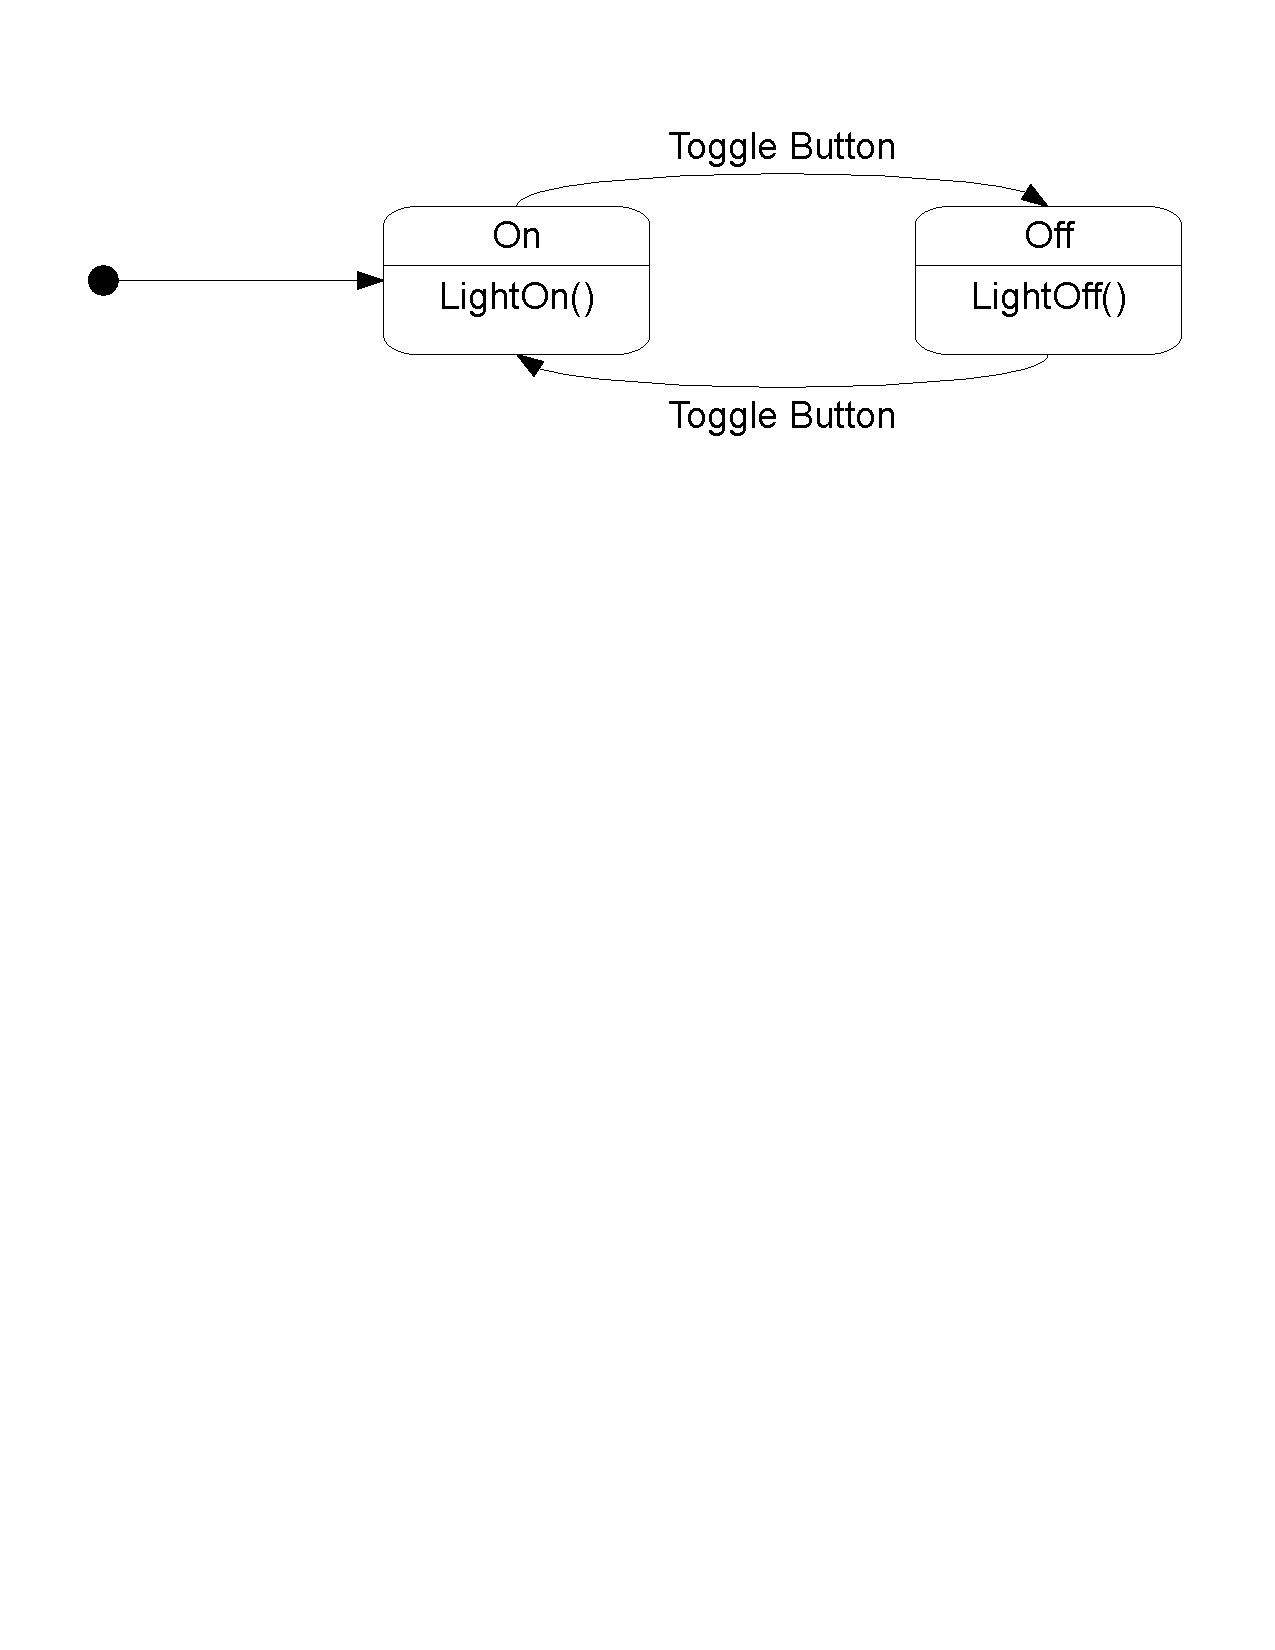
\includegraphics[trim= 15mm 200mm 15mm 10mm, clip, width=\imgmedium]{./images/state_uml_light.pdf} 
    \caption{UML State Chart of a Toggle Light}
    \label{fig:state_uml_light}
\end{figure}

The accepting state is defined in state charts as any states where inputs are accepted. In other words this is generally a state in which the machine has successfully performed its task and is now ready to take on another one. Accepting states generally can reach all other states in the system. The symbol for an accepting state is a state with a double outline, this is shown in figure \ref{fig:state_moore_mealy}. For our implementation we do not need to model this behaviour and therefor the concept of accepting states have been left out for practical purposes.

The UML defined state charts as shown in figure \ref{fig:state_uml_light} also allow for state titles in each state which can be seen at the top of each state. In addition, each state may contain executed actions that will occur. In this case "LightOn()" and "LightOff()" refer to executed routines that are called once the "On" and "Off" states are reached respectively. The behaviour is then once the state "On" is reached "LightOn()" is executed right away.

%diagram for UML state machines
\begin{figure}[htp]
    \centering
    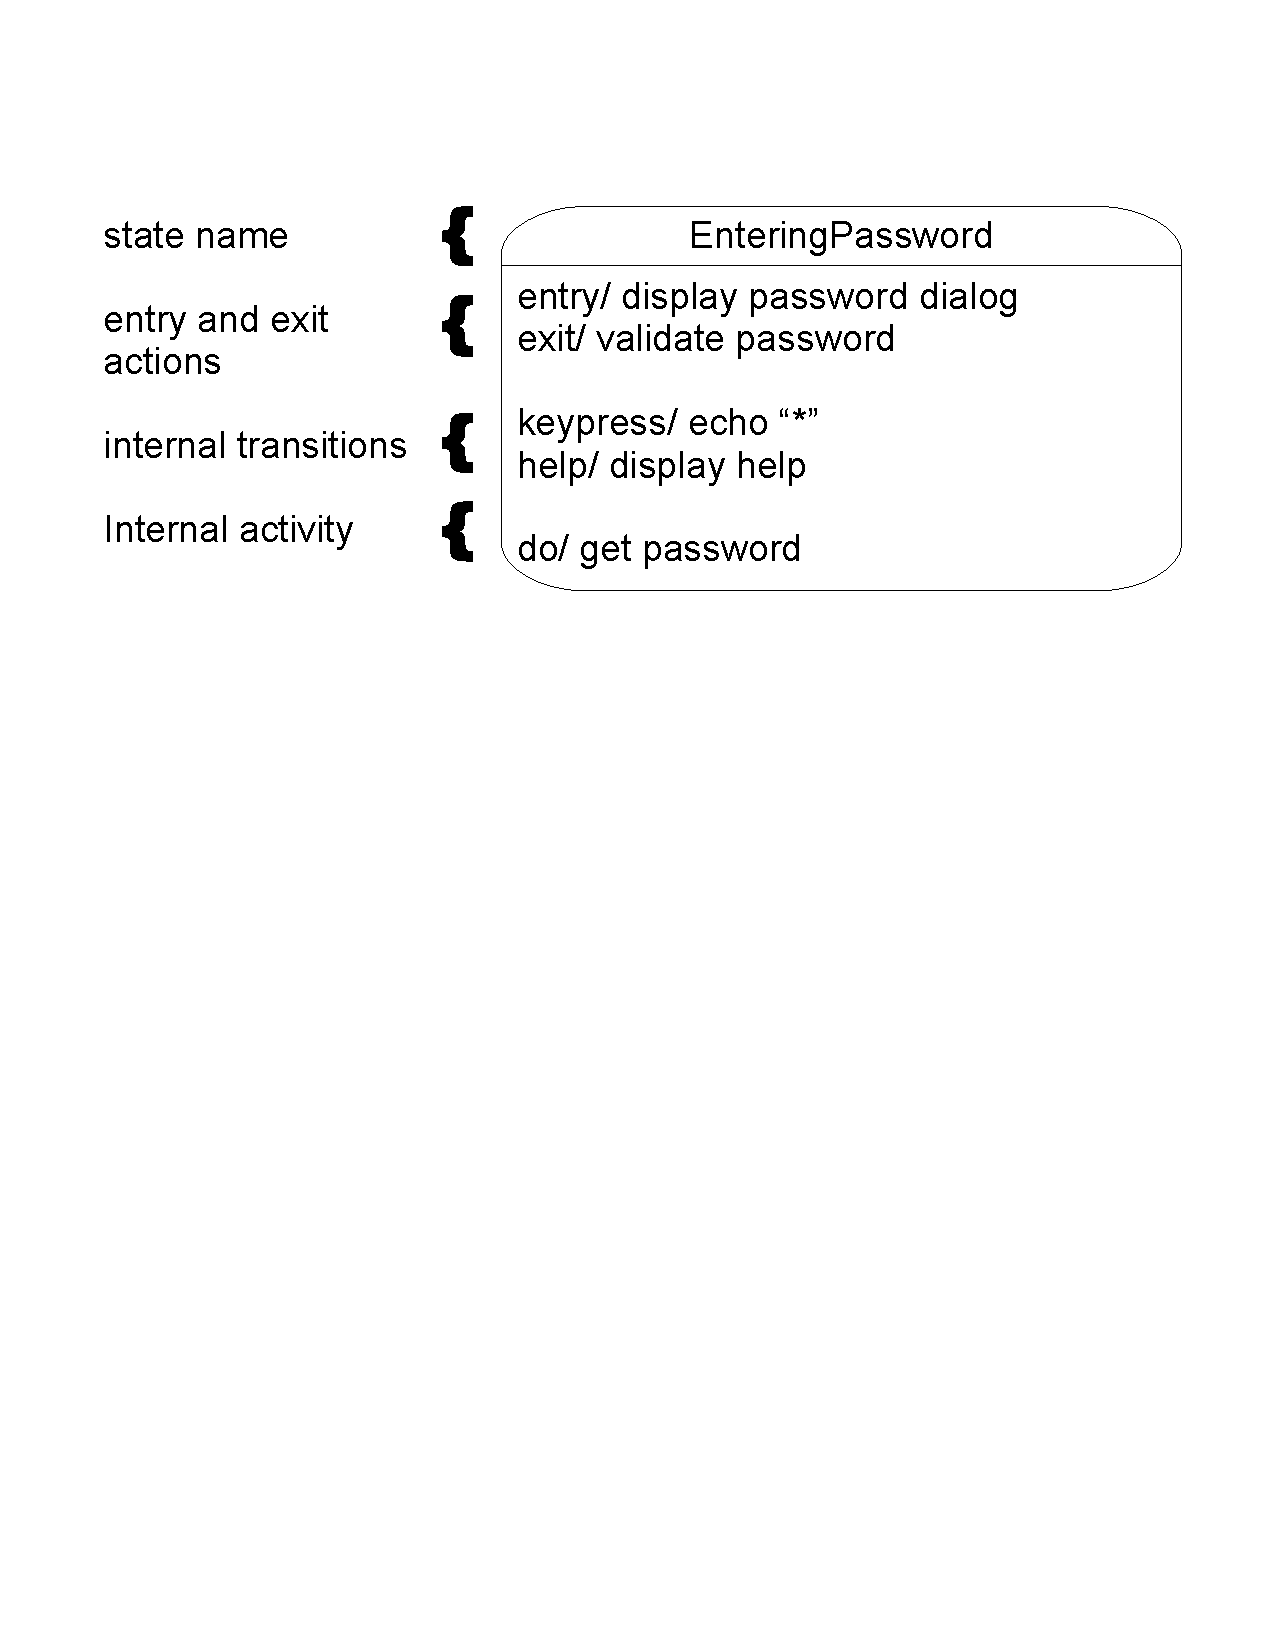
\includegraphics[trim= 15mm 175mm 15mm 10mm, clip, width=\imgmedium]{./images/state_uml2_syntax_21_4.pdf} 
    \caption{UML2 State Chart Syntax \cite{UML2}}
    \label{fig:state_uml2}
\end{figure}

The syntax shown in figure \ref{fig:state_uml_light} is UML2. UML2's specifications of state charts allows for additional information in each state. In figure \ref{fig:state_uml2} we note the additional features of UML2. Each state in UML2 can contain the following information. This inherent flexibility makes UML2 more useful for representing more practical programs. In addition UML2 has a more precise syntax when compared to other methods of describing state charts.

\begin{itemize}
	\item \textbf{state name:} The state name is mandatory for each UML2 state in cases where this is the only information the horizontal divider may be omitted.
	\item \textbf{entry and exit actions:} Entry and exit options are optional, they are commonly used for initializers and finalizers that may occur upon each state.
	\item \textbf{internal transitions:} These optional fields refer to simple transitions that may happen in the state itself generally these are simple enough to not require a separate diagram.
	\item \textbf{internal activity:} Also optional but refer to activities that occur or are executed while in the state.
\end{itemize}

